\section{Background}\label{section:background}

\subsection{Starcraft}

Starcraft is a \emph{Real Time Strategy} (RTS) game published by
Blizzard Entertainment. It follows the ``gather-build-conquer''
pattern, in which each player (human or AI) must gather resources
available in the play field to build combat units and
structures. These units are used to attack the other players,
destroying their units and structures and denying their access to
resources. The game features a wide variety of combat units, with
different speeds, attack range, strengths and weakenesses. The balance
between combat and resource gathering leads to the concepts of
\emph{micromanagement} (micro) and \emph{macromanagement}
(macro). Micro are the tactical actions and skills involving
individual battles between a game, while Macro are the strategic
decisions such as building management, resource usage, and unit
creation. A sucessful player (or bot) needs to eventually master
these two aspects of the game.

Development of AI agents for Starcraft is a vibrant research field
(See surveys by Onta\~non~\cite{Ontanon13AICompetitionSurvey} and
Certicky~\cite{Certicky17SurveyCompetitionsBots}). They highlight that, unlike Go and Chess,
Starcraft presents Game Playing AI the challenge of dealing with
real-time, partial information scenarios. Therefore, Starcraft is a
hard challenge for AI. An unofficial framework for the development of
AI agents exists in the form of the \emph{Brood Wars API}
(BWAPI)~\cite{BWAPI}. It allows the user to read and write to the
game's memory, allowing a wide range of agent types, from agents that
control limited parts of an AI opponent, to agents with the same range
of inputs and outputs as a human player.

% This requires good thinking, decision making and fast reactions.
% The game features three different races and all units are unique to
% their respective races, performs differently and requires different
% tactics.  The game is well known for being well balanced and as such
% was widely used in competitions.  Indeed even though each race is
% unique, has different strengths and abilities, their overall
% strength is the same and no race has an advantage over the
% other. This is because the game is now quite old and the balance
% have been polished over time via game updates provided by Blizzard
% Entertainment, developer and publisher of the game. It makes this
% game a great support to develop competitive, modular, adaptative
% agents.

% To create Starcraft: Broodwar agents, the \emph{BWAPI (Brood War
% Application Programming Interface) free and open source C++
% framework} is widely used by students, researchers and
% hobbyists. This framework isn't an official product from Blizzard
% and access and modify the game state by reading and writing directly
% the memory space of the game. As such is considered to be a "hack"
% that violates the End User License Agreement of the game. However,
% it is tolatered by company (and even encouraged given that they
% provided prizes to the tournament sponsorised by
% AIIDE\footnote{Artificial Intelligence and Interactive Digital
% Entertainment}). Reading / writing directly in the memory space of
% another program is considered to be an unsafe method (at least in
% term of stability) but the framework has been used and maintained
% for a long time and is considered stable.  It can be configured so
% as to only reveals the parts of the game state that are visibles by
% the agent, effectively providing only information that a real human
% player would have access to. That way, it is possible to write
% non-cheating AIs that operate under partial information conditions.

\subsection{Micromanagement}

In this study we focus on the \emph{Micromanagement} (Micro) aspect of
an Starcraft controller. Micro refers to the control of individual
units involved in a tactical combat. This involves sending commands to
each individual unit as a player would do, such as ``attack unit A'' or
``move to position X,Y''.

\begin{figure}
  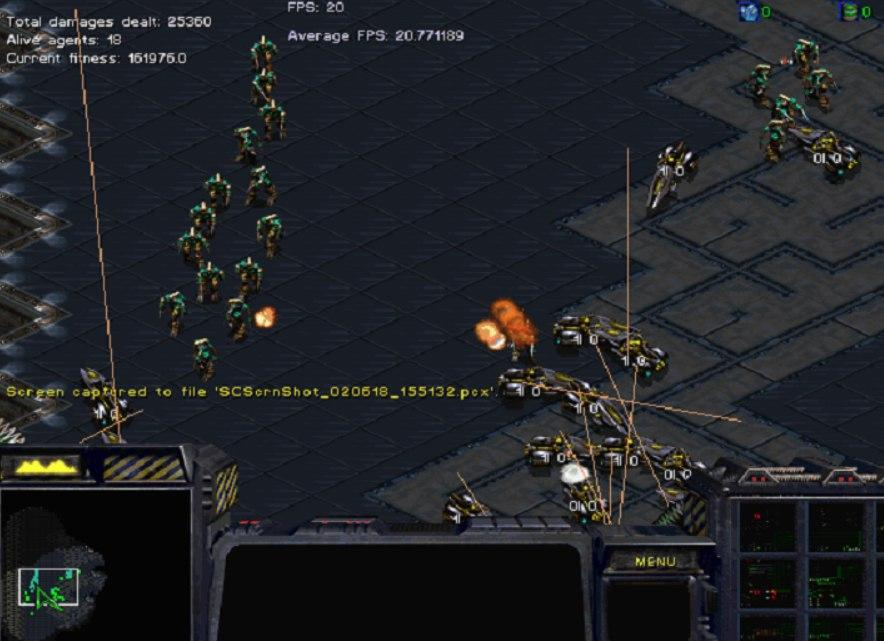
\includegraphics[width=.5\textwidth]{figures/vultures_vs_zealots_combat}
  \caption{Combat opposing vultures to zealots}\label{fig:combat-example}
\end{figure}

There are many approaches to developing Starcraft micro
controllers. Wender and Watson investigate the viability of
Reinforcement Learning to this task~\cite{Wender12ReinforcementMicroSC}. They show that a
variety of RL techniques could achieve 100\% win ratios in small
combat situations, by controlling two actions: ``Attack'' and
``Retreat''.

Shantia et al. explore the use of neural networks to also order a unit
to ``attack'' or ``flee''~\cite{Shantia11ConnectionistSC}. The weights of the neural
network are adjusted by a RL algorithm. They show that you can train
the neural network on smaller combats (3x3) to perform well in larger
engagements (6x6).

More recently, Neuro Evolution has become a popular approach for
training Starcraft controllers. Zhen and Watson show a comparison of
NEAT and rtNEAT~\cite{Zhen13NeuroEvoSC} for training a micro controller (also
using ``Attack'' and ``Retreat''). Their setup includes four classes
of engagement (ranged vs melee, melee vs melee, ranged vs ranged and
melee vs ranged), each with two teams of 12 units. They remark how the
unit composition of the match up has an effect on the variability of
the result.

One thing that all of these approaches (and a few others) have in
common is that the evaluation of the training is based on the win
ratio and the number of enemies killed. In this study, we want to
explore how to achieve a more ``humane'' behavior, i.e. achieving
victories while at the same time conserving the fighting force and
maximizing the number of surviving units.

\subsection{NEAT}\label{subsec:neat}

NEAT (\emph{Neuro Evolution of Augmented Topologies}) is a machine
learning technique which combines neural network and evolutionary
computation ideas to develop both the weights and the topology
(structure) of a neural network~\cite{Stanley02Neat}.

NEAT begins with a minimal topology, and grows it through training in
order to match the problem difficulty, adding and removing neurons and
connections and changing weights. Self connections and connections to
different layers are possible, which means that NEAT can evolve
recurrent neural networks. Additionally, NEAT includes a speciation
mechanism to promote genetic diversity in the population.

rtNEAT is a variant of NEAT for real time problems, which was
originally demonstrated on the combat game NERO. Since then, NEAT and
rtNEAT have been popular choices for the training of controllers in
tactical scenarios. The ability to match each unit to a separate
network in the population, and the ability to progressively learn more
complex behaviors are two compelling reasons for the use of
NEAT/rtNEAT in Starcraft.

Accordingly, recently variants of NEAT such as CascadeNEAT have also
been proposed to answer to specific problems.

\subsection{Cascade-NEAT}\label{subsec:cascade-neat}

Cascade-NEAT is a variant of NEAT which aims at restricting the neural
network search space to topologies that have a so-called cascade
architecture. A cascade architecture means that all hiden neurons are
connected to all other neurons, and only connections associated with
the most recently added hidden neuron are modified by the evolutionary
process.

Kohl~\cite{Kohl09FracturedProblems, Kohl09StrategicDecisions} reports that this method is good for
fractured problems, such as the concentric spiral clustering problem
and the keepaway soccer decision problem. However, Cascade-NEAT
performs very poorly on some problems requiring recurrent connectivity
patterns, since it cannot produce such patterns. An example of such
failure is the non-Markovian double pole-balancing problem for which
cascade-NEAT doesn't find a single suitable solution whereas the
standard NEAT performs very well.

To our knowledge, Cascade-NEAT has not been applied to the Starcraft
problem. Because of the similarity of some strategic decisions
involved in Starcraft micro management and the keepaway soccer problem
we decided to include Cascade-NEAt as one of the alternatives for the
current investigation.

\subsection{Novelty search}\label{subsec:novelty-search}

Novelty search is a new approach to planning and search algorithms
where, instead of rewarding the agents for progressing towards a fixed
objective, agents are rewarded for finding solutions that are different
from other solutions already found by the algorithm.

Surprisingly, sometimes not explicitly looking for the objective leads
to finding a solution faster, specially in the case of deceptive
problems.  Indeed, intermediate steps and partial solutions may
require an evolution towards a completely different direction than
that of the final expected result. In these cases, objective-oriented
algorithms may get stuck in local optima and cause the search to
fail.

\citet{Lehman11Novelty} demonstrated this with an experiment where a robot
controlled by a neural network has to find a specific location in a
maze. A solution's novelty is characterized by the end location of the
robot, compared to all others so far. Only Novelty Search was able to
find the goal in the deceptive maze.

\subsection{Potential fields}\label{subsec:potential-fields}

Potential Fields, also called Artificial Potential Fields (APF), is a
method using the idea of attracting and repelling fields in a
space. It is mainly used for planning tasks involving maneuvering.
The sum of all the fields given the agent's position is used to
determine the direction for its next move. The strength of a
particular field on the agent's movement is proportional to the
closeness of that agent to the field's center

This algorithm was originally used to make robots navigate between
obstacles. Obstacles are given a repelling fields while the objective
is given an attractive field. However, using it in RTS games has been
explored as well \cite{Hagelback08RTSPotentialFields}.
\citet{Svendsen12SCPotentialFieldsGP} applied this method to
StarCraft micromanagement along with a multi-objective evolutionary
algorithm called NSGA-II to optimize the fields automatically.
